\documentclass[10pt]{article}
\usepackage[utf8]{inputenc}
\usepackage[activeacute,spanish]{babel}
\usepackage[left=1.5cm,top=1.5cm,right=1.5cm, bottom=1.5cm,letterpaper, includeheadfoot]{geometry}

\usepackage{amssymb, amsmath, amsthm}
\usepackage{graphicx}
\usepackage{hyperref}
\usepackage{lmodern,url}
\usepackage{paralist} %util para listas compactas
\usepackage{xcolor}

%========PAQUETES AGREGADOS===========
%Pseudocodigo
\usepackage{pseudocode}
\usepackage[portuguese, boxruled]{algorithm2e}
\usepackage{wrapfig}
\usepackage{multicol}
\usepackage{graphicx}
\usepackage{caption}
\usepackage{subcaption}
%\captionsetup[table]{labelformat=empty}
\captionsetup[subfigure]{labelformat=empty}
\usepackage{cancel}
%====================================

\usepackage{fancyhdr}
\pagestyle{fancy}
\fancypagestyle{plain}{%
\fancyhf{}
\lhead{\footnotesize\itshape\bfseries\rightmark}
\rhead{\footnotesize\itshape\bfseries\leftmark}
}


% macros
\newcommand{\Q}{\mathbb Q}
\newcommand{\R}{\mathbb R}
\newcommand{\N}{\mathbb N}
\newcommand{\Z}{\mathbb Z}
\newcommand{\C}{\mathbb C}
\newcommand{\BigO}{\mathcal{O}}
%Teoremas, Lemas, etc.
\theoremstyle{plain}
\newtheorem{teo}{Teorema}
\newtheorem{lem}{Lema}
\newtheorem{prop}{Proposición}
\newtheorem{cor}{Corolario}
\newtheorem{obs}{Observación}
\newtheorem{ej}{Ejemplo}
\renewcommand{\qedsymbol}{\rule{0.7em}{0.7em}}
\renewenvironment{proof}{{\bfseries \noindent Demostración}}{ \qed \\}


\theoremstyle{definition}
\newtheorem{defi}{Definición}
% fin macros


\newcommand{\catnum}{2} %numero de catedra
\newcommand{\fecha}{6 de Septiembre 2016 }

%%%%%%%%%%%%%%%%%%

%Macros para este documento
\newcommand{\cin}{\operatorname{cint}}



\begin{document}
%Encabezado
\fancyhead[L]{Facultad de Ciencias Físicas y Matemáticas}
\fancyhead[R]{Universidad de Chile}
\vspace*{-1.2 cm}
\begin{minipage}{0.6\textwidth}
\begin{flushleft}
\hspace*{-0.5cm}\textbf{MA3402-1 Estadística. Primavera 2016}\\
\hspace*{-0.5cm}\textbf{Profesor:} Raul Gouet\\
\hspace*{-0.5cm}\textbf{Escriba:} Manuel Cáceres\\
\hspace*{-0.5cm}\textbf{Fecha:} \fecha
\end{flushleft}
\end{minipage}
\begin{minipage}{0.36\textwidth}
\begin{flushright}

\includegraphics[scale=0.3]{imagenes/fcfm_dcc}
\end{flushright}
\end{minipage}
\bigskip
%Fin encabezado

\begin{center}
\LARGE\textbf{Clase \catnum}
\end{center}

Tenemos un modelo que consiste en una familia $\mathcal{P}$ de medida de probabilidad sobre $(\Omega, \mathcal{F})$.\\

Escribimos:
\begin{itemize}
\item $\mathcal{P}=\{\mathbb{P}_{\theta}\colon \theta \in \Theta \}$, en donde a $\theta$ le llamamos parámetro del modelo y $\Theta$ espacio de parámetros.
\end{itemize}
Cuando $\Theta \subseteq \mathbb{R}^k$, tenemos $\theta = (\theta_{1}, \theta_{2}, \ldots, \theta_{k})$ y los $\theta_{i}$ son parámetros reales. En este caso diremos que nuestro modelo es paramétrico (pues hay un número finito de parámetros).\\

Para nosotros $\theta$ es un parámetro fijo desconocido.\\
Podemos observar $X$ (que es un objeto aleatorio) a valores en $\mathfrak{X}$ (espacio medible, típicamente $\mathbb{R}^n$).
\begin{align*}
X \colon (\Omega, \mathcal{F}, ?) \mapsto (\mathfrak{X}, \mathcal{B}(\mathfrak{X}), inducida)
\end{align*}

Supondremmos que está actuando una probabilidad $\mathbb{P}_{\theta} \in \mathcal{P}$, pero no sabemos cual. Queremos adivinar cual es en base a la observación de $X$.\\

Si hemos visto $X=x$, entonces postularemos que la probabilidad en acción es tal.\\

El problema de estimación consiste en usar la información entregada por $X$ para calcular aproximadamente(estimar) una función $g(\theta)$ del parámetro. Esto se consigue definiendo los estadísticos y estimadores.

\section{Estadístico}
Se define como estadístico a cualquier función medible $T: \mathfrak{X} \mapsto \mathcal{T}$(otro espacio medible).
El estadístico $T$ puede servir para ``resumir'' la información.\\

Por ejemplo, si $\mathfrak{X} = \mathbb{R}^n,\ x = (x_{1}, x_{2}, \ldots, x_{n})$ entonces son estadísticos:
\begin{itemize}
\item $T(x) = \sum_{i=1}^n{x_{i}}$
\item $S(x) = max\{x_{1}, x_{2}, \ldots, x_{n}\}$
\item $H(x) = \left(\sum_{i=1}^n{x_{i}}, \sum_{i=1}^n{x_{i}^2}\right)$
\end{itemize}
Estos estadísticos son muy comunes.\\

Por extensión diremos que la variable aleatoria $T(X)$ (composición) es un estadístico.

\section{Estimador}
Un estimador de $g(\theta)$ es un estadístico (habitualmente denotado $\hat{g}$ o $\tilde{g}$)	cuyos valores se parezcan a $g(\theta)$. También diremos que $\hat{g}(X)$ es estimador. Pero a los valores $\hat{g}(x)$ les llamaremos estimaciones.

\begin{ej} Modelo de Bernoulli con $\theta \in \left[0,1\right],\ X = (X_{1}, X_{2}, \ldots, X_{n}),\ \mathfrak{X} = \{0,1\}^n$.\\
Donde $\mathbb{P}_{\theta}\left[X=x\right] = \theta^{\sum{x_{i}}}(1-\theta)^{n-\sum{x_{i}}}$.\\
Sea $T(x) = \sum_{i=1}^n{x_{i}}$ un estadístico, y $g(\theta) = \theta$ la función a estimar.\\

Sean $\hat{g_{1}}(x) = \frac{1}{n}\sum_{i=1}^n{x_{i}} = \frac{1}{n}T(x)$ y $\hat{g_{2}}(x) = x_{1}$ dos estimadores de $g(\theta)$.\\
Si observamos $x=(1,1,0,0,1,0)$ entonces $\hat{g_{1}}((1,1,0,0,1,0)) = \frac{1}{2}$ y $\hat{g_{2}}((1,1,0,0,1,0)) = 1$ son dos estimaciones de $\theta (g(\theta))$.\\
\end{ej}
¿Cómo medimos la calidad de un estimador?

\section{Calidad de un estimador}
Definamos un estimador ideal de $g(\theta)$.\\
 Diremos que $\hat{g}$ es un estimador ideal o perfecto si
 \begin{align*}
 \mathbb{P}_{\theta}(\hat{g}(X) = g(\theta)) = 1,\ \forall \theta \in \Theta
 \end{align*}
Tales estimadores no existen en general, salvo casos artificiales.\\

Por ejemplo, supongamos que $\mathfrak{X}$ se particiona como $\mathfrak{X} = \{\mathfrak{X}_{\theta}\colon \theta \in \Theta\}$ y tal que $\mathbb{P}_{\theta}(X \in \mathfrak{X}_{\theta}) = 1$. En tal caso podemos construir un estimador perfecto de $g(\theta)$, porque basta saber que $X$ toma valor en $\mathfrak{X}_{\theta_{0}}$ para decir que $g(\theta)$ es $g(\theta_{0})$.\\
Esto no es realista porque distinos valores de $\theta$ pueden producir el mismo valor de $X$.\\
Hay que proponer otras formas de evaluar estimadores.\\
Supongamos que $g(\theta)$ es a valores reales y que $\hat{g}$, el estimador de $g(\theta)$ es a valores reales.

\section{Error Cuadrático Medio}
Sea $\hat{g}(X)$ un estimador de $g(\theta)$, se define su error cuadrático medio como:
\begin{align*}
ecm_{\theta}(\hat{g(X)}) = \mathbb{E}_{\theta}\left[(\hat{g}(X) - g(\theta))^2\right]\ &\quad \text{posiblemente infinito}
\end{align*}
Esto es una función de $\theta \mapsto ecm_{\theta}(\hat{g})$.\\

Podemos decir que $\hat{g_{1}}$ es mejor estimador de $g(\theta)$ que $\hat{g_{2}}$ si:
\begin{align*}
ecm_{\theta}(\hat{g_{1}}) \le ecm_{\theta}(\hat{g_{2}})\ ,\quad \forall \theta \in \Theta
\end{align*}
\begin{center}
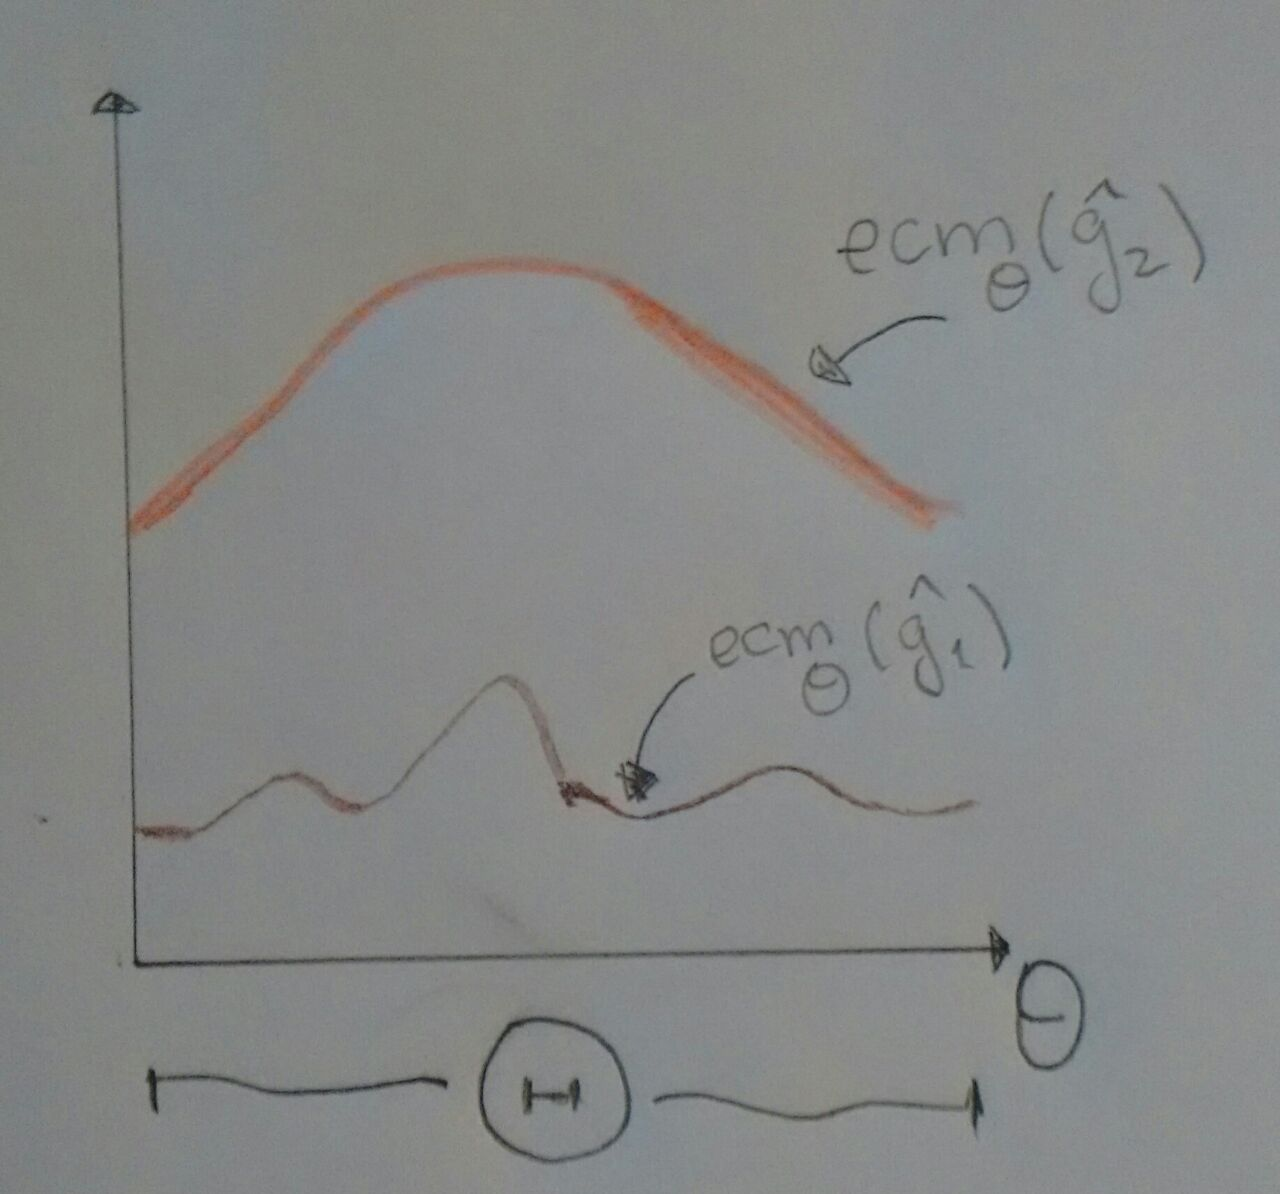
\includegraphics[scale=0.1]{imagenes/ecm.jpg}
\end{center}
Podemos definir la optimalidad de un estimador $\hat{g}^*$, diciendo que s óptimo para el $ecm$ si:
\begin{align*}
ecm_{\theta}(\hat{g}^*) \le ecm_{\theta}(\hat{g})\ ,\quad \forall \theta \in \Theta,\ \forall \hat{g}, \text{estimador de $g(\theta)$}
\end{align*}
Salvo situaciones artificiales no existen estimadores óptimos globalmente para el $ecm$.\\

Para verificarlo pensemos en el siguiente estimador(absurdo):
\begin{align*}
\tilde{g}(x) = g(\theta_{0}),\ &\quad \text{para algún $\theta_{0} \in \Theta$ fijo}
\end{align*}
Ocurre que $ecm_{\theta}(\tilde{g}) = (g(\theta_{0})-g(\theta))^2$, entonces $ecm_{\theta_{0}}(\tilde{g}) = 0$, luego necesariamente $\hat{g}^*$ tiene que tener $ecm_{\theta_{0}}(\hat{g}^*) = 0$, pero como $\theta_{0}$ es cualquiera, entonces en realidad estamos pidiendo $ecm_{\theta}(\hat{g}^*) = 0,\ \forall \theta \in \Theta$, que es equivalente a pedir $\mathbb{P}_{\theta}(\hat{g}^*(X) = g(\theta)) = 1,\ \forall \theta \in \Theta$.\\

La solución consiste en considerar clases de estimadores que no contengan casos como $\tilde{g}(x) = g(\theta_{0})$.

\section{Sesgo e Insesgamiento}
En lo que sigue $\hat{g}(X)$ es un estimador de $g(\theta)$. Ambas funciones podrían ser con valores en $\mathbb{R}^p$ (o incluso Banach).\\
Se define el sesgo de $\hat{g}(X)$, como estimador de $g(\theta)$, mediante :
\begin{align*}
\mathfrak{b}_{\theta}(\hat{g}) = \mathbb{E}_{\theta}(\hat{g}(X)) - g(\theta)
\end{align*}

Se dice que $\hat{g}$ es insesgado si $\mathfrak{b}_{\theta}(\hat{g}) = 0$ o bien $\mathbb{E}_{\theta}(\hat{g}(X)) = g(\theta)$, $\forall \theta \in \Theta$.\\

En el caso de un estimador $\hat{g}$ insesgado para $g(\theta)$, se tiene (cuando existe) (aquí volvemos a $g(\theta)$ con valores en $\mathbb{R}$)
\begin{align*}
ecm_{\theta}(\hat{g}) &= \mathbb{E}_{\theta}((\hat{g}(X)-g(\theta))^2)\\
&= \mathbb{E}_{\theta}((\hat{g}(X)-\mathbb{E}_{\theta}(\hat{g}(X)))^2)\\
&= \mathbb{V}_{\theta}(\hat{g}(X))
\end{align*}

Dentro de la clase de los esimadores insesgados para $g(\theta)$, buscamos aquel con mínimo $ecm$ (óptimo), es decir, con mínima varianza. Buscaremos, en diversos modelos, los estimadores insesgados de varianza uniformemente mínima (EIVUM).

\begin{ej} Modelo de Bernoulli \\
\begin{align*}
\mathbb{P}_{\theta}(X=x) = \theta^{\sum{x_{i}}}(1-\theta)^{n-\sum{x_{i}}},\ &\quad x = (x_{1}, x_{2}, \ldots, x_{n}) \in \mathfrak{X}=\{0,1\}^n,\ \theta \in \Theta = \left[0,1\right]\\
g(\theta) = \theta,\ \hat{g}(X) = \frac{1}{n}\sum{X_{i}}\\
\mathbb{E}_{\theta}(\hat{g}(X)) = \mathbb{E}_{\theta}(\frac{1}{n}\sum_{i=1}^n{X_{i}}) &= \frac{1}{n}\sum_{i=1}^n\mathbb{E}_{\theta}(X_{i})= \frac{1}{n}\sum_{i=1}^n\mathbb{P}_{\theta}(X_{i} = 1)\\
&= \frac{1}{n}\sum_{i=1}^n\theta = \theta = g(\theta)
\end{align*}
Entonces $\bar{X}_{n} = \frac{1}{n}\sum_{i=1}^nX_{i}$ es un estimador insesgado de $g(\theta) = \theta$.
\end{ej}

\begin{ej} Modelo Gaussiano \\
Consideremos $\mathfrak{X} = \mathbb{R}^n$ y $x = (X_{1}, X_{2}, \ldots, X_{n})$ con densidad (de $X$):
\begin{align*}
f_{\theta}(x) = \left(\frac{1}{\sqrt{2\pi}\sigma}\right)^ne^{-\frac{1}{2}\sum{\left(\frac{x_{i}-\mu}{\sigma}\right)^2}},\ &\quad \theta = (\mu, \sigma) \in \Theta = \mathbb{R}\times (0,\infty)
\end{align*}
Si queremos estimar $g(\theta) = \mu$ se puede considerar $\hat{g}(X) = \frac{1}{n}\sum{x_{i}}$ porque :
\begin{align*} %% Revisar esto último
\mathbb{E}_{\theta}(\hat{g}(X)) = \mathbb{E}_{\theta}\left(\frac{1}{n}\sum x_{i}\right) = \frac{1}{n}\mathbb{E}_{\theta}(X_{i})\quad \text{con}\\
\mathbb{E}_{\theta}(X_{i})= \int_{-\infty}^{\infty}{\frac{x}{\sqrt{2\pi}\sigma}e^{-\frac{1}{2}\left(\frac{x-\mu}{\sigma}\right)^2}dx} = \mu
\end{align*}
\end{ej}
\end{document}